\documentclass{beamer}

\mode<presentation> {
    \usetheme{default}
}

\setbeamertemplate{caption}[numbered]

\makeatletter
\setbeamertemplate{footline}{%
  \leavevmode%
  \hbox{%
  \begin{beamercolorbox}[wd=.5\paperwidth,ht=2.25ex,dp=1ex,right]{date in head/foot}%
   %\insertframenumber{} / \inserttotalframenumber\hspace*{2ex} % old version
    \insertframenumber{} \hspace*{2ex} % new version without total frames
  \end{beamercolorbox}}%
  \vskip0pt%
}
\makeatother

\usepackage{graphicx} % Allows including images
\usepackage{booktabs} % Allows the use of \toprule, \midrule and \bottomrule in tables
\usepackage{ctex}
\usepackage{listings}
\usepackage{color}
\usepackage[font=scriptsize,labelfont=bf]{caption}
\usepackage{tikz}
\usetikzlibrary{positioning, shapes.geometric}

\lstset {
    basicstyle={\scriptsize\ttfamily},
    frame=shadowbox,
    breaklines=true
}

% 流程图定义基本形状
\tikzstyle{startstop} = [rectangle, rounded corners, minimum width=3cm, minimum height=0.5cm,text centered, draw=black, fill=red!30]
\tikzstyle{io} = [trapezium, trapezium left angle=70, trapezium right angle=110, minimum width=3cm, minimum height=1cm, text centered, draw=black, fill=blue!30]
\tikzstyle{process} = [rectangle, minimum width=3cm, minimum height=0.5cm, text centered, draw=black, fill=orange!30]
\tikzstyle{decision} = [diamond, minimum width=3cm, minimum height=1cm, text centered, draw=black, fill=green!30]
\tikzstyle{arrow} = [thick,->,>=stealth]

%----------------------------------------------------------------------------------------
%	TITLE PAGE
%----------------------------------------------------------------------------------------

\title[]{Linux 启动流程} % The short title appears at the bottom of every slide, the full title is only on the title page

\author{伍华龙} % Your name
\date{\today} % Date, can be changed to a custom date

\begin{document}

\begin{frame}
    \titlepage % Print the title page as the first slide
\end{frame}

\begin{frame}
    \frametitle{目录}
    \begin{itemize}
        \item Linux 概述
        \item Linux 启动流程概述
        \item UEFI
        \item Boot loader
        \item Kernel
        \item Init process
    \end{itemize}
\end{frame}

%----------------------------------------------------------------------------------------
%	PRESENTATION SLIDES
%----------------------------------------------------------------------------------------

\section{Linux 概述}

\begin{frame}
    \frametitle{Linux 概述}
    \begin{itemize}
        \item 操作系统是什么
        \item 操作系统的组成
        \item Linux 简史
    \end{itemize}
\end{frame}

\begin{frame}
    \frametitle{操作系统是什么}
    \begin{itemize}
        \item 操作系统是大型的、复杂的和长寿命的程序。
        \item 操作系统主要执行两个任务:
        \begin{itemize}
            \item 提供接口。隐藏硬件,为程序员提供方便的接口——系统调用。
            \item 管理资源。管理处理器、存储器、I/O接口设备等。
        \end{itemize}
    \end{itemize}

    \begin{figure}[htbp]
    \centering
    \begin{minipage}[t]{0.48\textwidth}
    \centering
    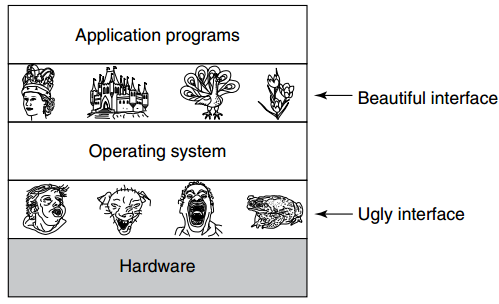
\includegraphics[width=5cm]{images/os_interface.png}
    \caption{Operating systems turn ugly hardware into beautiful abstractions}
    \end{minipage}
    \end{figure}
\end{frame}

\begin{frame}
    \frametitle{操作系统的组成}
    \begin{itemize}
        \item 进程管理
        \item 内存管理
        \item 文件系统
        \item I/O
        \item 安全
        \item ......
    \end{itemize}
\end{frame}

\begin{frame}
    \frametitle{Linux 简史(正经篇)}
    \footnotesize
    \begin{itemize}
        \item 1969年8月,美国贝尔实验室的Ken Thompson写了第一个版本的Unix。
        \item 1973年,Dennis Ritchie和Ken Thompson使用C语言重写了Unix。
        \item 1974年,Dennis Ritchie和Ken Thompson发布论文,首次公开Unix。
        \item 1987年,Andrew Tanenbaum写了Minix,用于操作系统教学。
        \item 1991年,Linus Torvalds写了Linux v0.0.2,并对外宣布Linux项目。
        \item 1992年,Linux内核在GNU GPL下被重新授权使用,产生第一个Linux发行版本。
    \end{itemize}

    \begin{figure}[htbp]
    \centering
    \begin{minipage}[t]{0.48\textwidth}
    \centering
    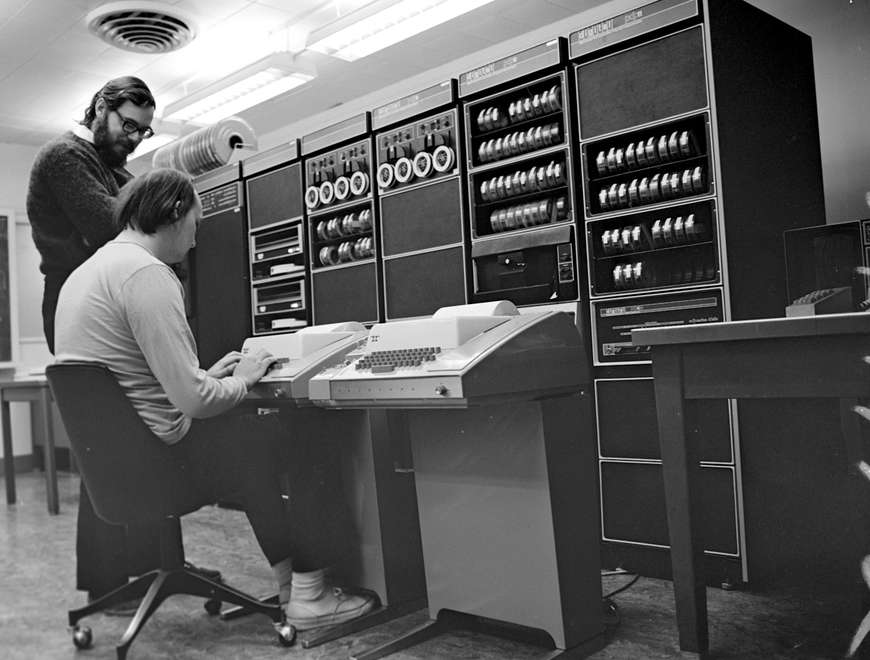
\includegraphics[width=5cm]{images/thompson_and_ritchie.jpg}
    \caption{Ritchie Dennis and Ken Thompson}
    \end{minipage}
    \begin{minipage}[t]{0.48\textwidth}
    \centering
    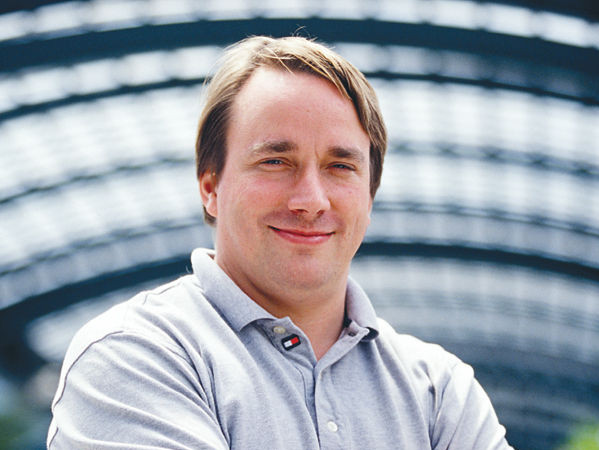
\includegraphics[width=5cm]{images/linus_torvalds.jpg}
    \caption{Linus Torvalds}
    \end{minipage}
    \end{figure}
\end{frame}

\begin{frame}
    \frametitle{Linux 简史(八卦篇)}

    \footnotesize
    \begin{itemize}
        \item 1969年,为了在一台旧的PDP-7机器上继续玩自己写的“星际旅行”游戏,Ken Thompson最终开发出Unix系统。
        \item 在妻儿去探亲的一个月内,Ken Thompson用汇编语言写出了Unix系统的原型。
        \item 1983年,Dennis Ritchie和Ken Thompson因为发明了Unix和C语言而获得图灵奖。
        \item 1991年,当Linus Torvalds写出Linux的第一个版本时,他还在芬兰的赫尔辛基大学读书,年仅22岁。
        \item 2005年,由于不能继续免费使用BitKeeper,Linus Torvalds在两周内开发出Git的最初版本。
        \item 2007年,Ken Thompson、Rob Pike和Robert Griesemer共同发明了Go语言。
    \end{itemize}
\end{frame}

\section{Linux 启动流程概述}

\begin{frame}
    \frametitle{Linux 启动流程概述}
    \begin{figure}
    \centering
    \begin{tikzpicture}[node distance=10pt]
        \node[startstop]                                       (start)   {上电};
        \node[process, below=of start]                         (step 1)  {UEFI 初始化硬件、加载 Boot loader};
        \node[process, below=of step 1]                        (step 2)  {Boot loader 显示启动菜单、加载 Kernel};
        \node[process, below=of step 2]                        (step 3)  {Kernel 解压、初始化、创建 Init 进程};
        \node[process, below=of step 3]                        (step 4)  {Init 进程启动各种用户态进程};

        \draw[arrow] (start)  -- (step 1);
        \draw[arrow] (step 1) -- (step 2);
        \draw[arrow] (step 2) -- (step 3);
        \draw[arrow] (step 3) -- (step 4);
    \end{tikzpicture}
    \caption{Linux 启动流程}
    \end{figure}
\end{frame}

\section{UEFI}

\begin{frame}
    \frametitle{UEFI}

    \begin{itemize}
        \item BIOS vs UEFI
        \item UEFI 启动流程
        \item 问题1:上电后 CPU 如何开始运行 UEFI?
        \item 问题2:UEFI 如何找到 boot loader?
    \end{itemize}
\end{frame}

\begin{frame}
    \frametitle{BIOS vs UEFI}
    \begin{itemize}
        \item Firmware: 固件
        \item Basic Input/Output System (BIOS): 基本输入输出系统
        \item Unified Extensible Firmware Interface (UEFI): 统一可扩展固件接口
    \end{itemize}

    \begin{table}
    \footnotesize
    \begin{center}
    \begin{tabular}{|c|c|c|}
    \hline
     & BIOS & UEFI \\ \hline
    开发效率 & 汇编代码,与硬件耦合度强,开发效率低 & C代码,接口统一,开发效率高 \\ \hline
    性能 & 中断+同步操作,性能差 & 事件+异步操作,性能高 \\ \hline
    扩展性 & 静态链接,扩展性差,升级慢 & 模块化设计,动态加载,升级简单 \\ \hline
    安全性 & 不考虑安全问题 & 支持安全启动功能 \\ \hline
    \end{tabular}
    \end{center}
    \caption{UEFI vs BIOS}
    \end{table}

\end{frame}

\begin{frame}
    \frametitle{UEFI 启动流程}
    \begin{figure}[htbp]
    \centering
    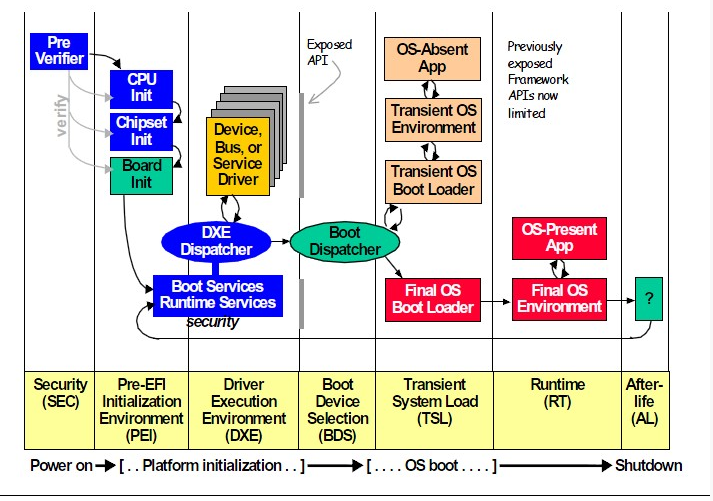
\includegraphics[width=6cm]{images/uefi_phases.png}
    \caption{UEFI系统的7个阶段}
    \end{figure}

    Questions:
    \begin{itemize}
        \footnotesize
        \color{red}
        \item 上电后CPU如何开始运行UEFI?
        \item UEFI如何找到boot loader?
    \end{itemize}
\end{frame}

\begin{frame}
    \frametitle{问题1:上电后CPU如何开始运行UEFI?}
    \begin{figure}
    \centering
    \begin{tikzpicture}[node distance=10pt]
        \node[startstop]                                       (start)   {按下电源开关};
        \node[process, below=of start]                         (step 1)  {电源给主板供电,并发送Power good signal给主板};
        \node[process, below=of step 1]                        (step 2)  {主板向CPU的reset引脚发送信号};
        \node[process, below=of step 2]                        (step 3)  {CPU清除所有寄存器的数据并设置为预定值(Reset vector)};
        \node[process, below=of step 3]                        (step 4)  {CPU执行第一条指令,该指令为跳转指令,跳转到UEFI的起始处};

        \draw[arrow] (start)  -- (step 1);
        \draw[arrow] (step 1) -- (step 2);
        \draw[arrow] (step 2) -- (step 3);
        \draw[arrow] (step 3) -- (step 4);
    \end{tikzpicture}
    \caption{由上电到开始运行UEFI}
    \end{figure}
\end{frame}

\begin{frame}
    \frametitle{问题2:UEFI如何找到boot loader?}

    \begin{itemize}
        \item UEFI 支持3个基本功能:
        \begin{itemize}
            \item 能够读 GPT 分区表
            \item 能够访问VFAT文件系统的文件
            \item 能够执行指定格式的可执行文件(EFI executables)
        \end{itemize}
        \item 在寻找boot loader时,UEFI 需要访问:
        \begin{itemize}
            \item UEFI boot manager
            \item GUID Partition Table (GPT)
            \item EFI system partitions (ESP)
        \end{itemize}
    \end{itemize}


\end{frame}

\begin{frame}[fragile]
    \frametitle{UEFI 启动管理器}
    \begin{itemize}
        \item 启动顺序、启动项等配置信息保存在 Non-Volatile Random Access Memory (NVRAM) 中。
        \item Linux 系统下,可以使用efibootmgr工具查询或更改启动顺序、启动项等配置。
    \end{itemize}

    \scriptsize
    \begin{lstlisting}
    along:~$ efibootmgr -v
    BootCurrent: 0000
    Timeout: 0 seconds
    BootOrder: 0000,0001,0017,0018,0019,001A,001B,001C,001D,001E
    Boot0000* ubuntu    HD(2,GPT,6470434e-fff7-4b5d-bd1b-a20975a1b0b6,
        0xfa000,0x31800)/File(\EFI\ubuntu\shimx64.efi)
    Boot0001* Windows Boot Manager  HD(2,GPT,6470434e-fff7-4b5d-bd1b-a20975a1b0b6,
        0xfa000,0x31800)/File(\EFI\Microsoft\Boot\bootmgfw.efi)WINDOWS
    \end{lstlisting}
\end{frame}

\begin{frame}
    \frametitle{GUID Partition Table (GPT)}
    \footnotesize
    \begin{itemize}
        \item 寻址方式:逻辑区块地址(Logical Block Address, LBA)
        \item GPT分配64 bits给逻辑区块地址,最大分区数为 $(2^{64} -1)$,若扇区大小为512 bytes,则总大小为 $(9.4 * 10^{21})$ bytes.
        \item 为减少分区表损坏的风险,GPT在硬盘最后保存了一份分区表的副本。
    \end{itemize}

    \begin{figure}[htbp]
    \centering
    \begin{minipage}[t]{0.48\textwidth}
    \centering
    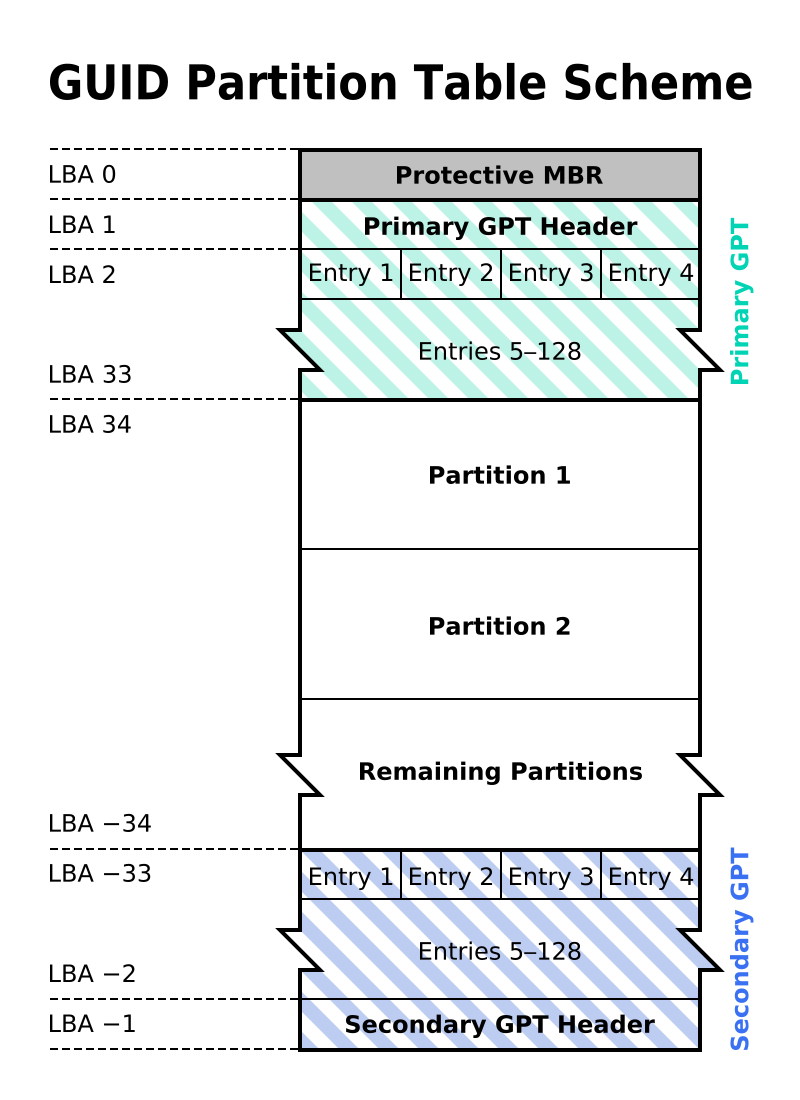
\includegraphics[width=5cm, height=5cm]{images/GUID_Partition_Table_Scheme.png}
    \caption{GPT的结构}
    \end{minipage}
    \begin{minipage}[t]{0.48\textwidth}
    \centering
    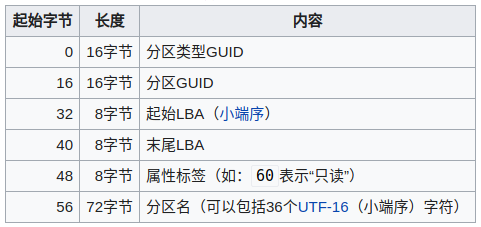
\includegraphics[width=5cm]{images/gpt_entry_format.png}
    \caption{GPT 分区表项的格式}
    \end{minipage}
    \end{figure}
\end{frame}

\begin{frame}
    \frametitle{EFI System Partition (ESP)}

    \begin{figure}[htbp]
    \centering
    \begin{minipage}[t]{0.48\textwidth}
    \centering
    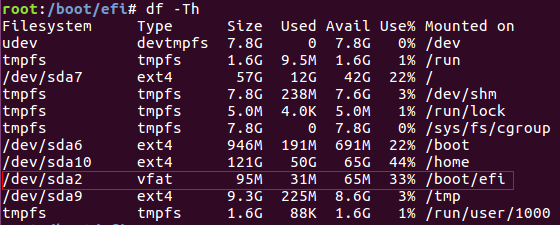
\includegraphics[width=5cm]{images/efi_filesystem.png}
    \caption{ESP 文件系统类型}
    \end{minipage}
    \begin{minipage}[t]{0.48\textwidth}
    \centering
    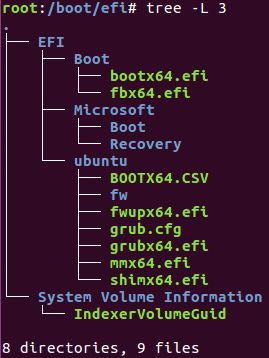
\includegraphics[width=3cm]{images/efi_tree.png}
    \caption{ESP 目录结构}
    \end{minipage}
    \end{figure}
\end{frame}

\begin{frame}
    \frametitle{回答:UEFI如何找到boot loader?}
    \begin{itemize}
        \item UEFI查询NVRAM中的启动配置信息,得到boot loader所在分区的GUID及分区下的相对路径。
        \item UEFI根据分区的GUID查询分区表,找到boot 所在的分区,再根据相对路径即可找到boot loader。
    \end{itemize}
\end{frame}

\section{Boot loader}

\begin{frame}
    \frametitle{Boot loader}

    GNU GRUB (GNU  GRand Unified Bootloader) 是大部分Linux发行版的默认boot loader,本章的讨论均以 GRUB2 为例。
    \vfill{}

    \begin{itemize}
        \item GRUB2 引导流程
        \item 问题3:GRUB2 如何找到 Kernel?
        \item 问题4:initrd.img 是什么?有什么用?
        \item x86 CPU 工作模式
    \end{itemize}
\end{frame}

\begin{frame}
    \frametitle{GRUB2 引导流程}
    \begin{figure}
    \centering
    \begin{tikzpicture}[node distance=10pt]
        \node[startstop]                                       (start)   {UEFI 将控制权交给 GRUB2};
        \node[process, below=of start]                         (step 1)  {GRUB2 显示启动菜单};
        \node[process, below=of step 1]                        (step 2)  {加载内核程序 vmlinuz};
        \node[process, below=of step 2]                        (step 3)  {加载文件系统镜像 initrd.img};
        \node[process, below=of step 3]                        (step 4)  {跳转到内核实模式代码的起始处};

        \draw[arrow] (start)  -- (step 1);
        \draw[arrow] (step 1) -- (step 2);
        \draw[arrow] (step 2) -- (step 3);
        \draw[arrow] (step 3) -- (step 4);
    \end{tikzpicture}
    \caption{GRUB2 引导流程概览}
    \end{figure}
\end{frame}

\begin{frame}
    \frametitle{显示启动菜单}
    UEFI 和 GRUB2 均提供显示和修改启动顺序的功能。

    \begin{figure}[htbp]
    \centering
    \begin{minipage}[t]{0.48\textwidth}
    \centering
    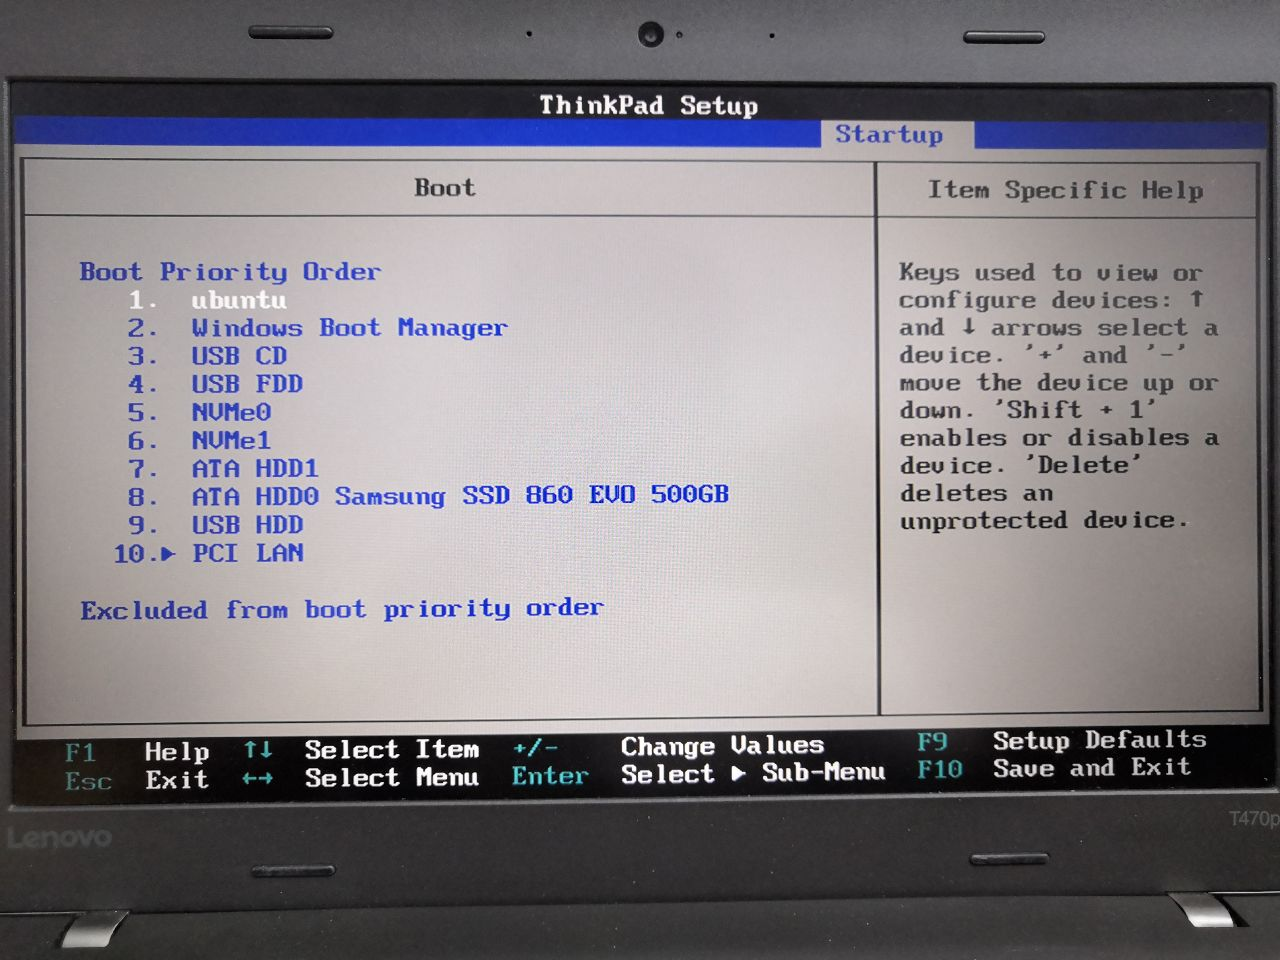
\includegraphics[width=5cm]{images/uefi_menu.jpg}
    \caption{UEFI 启动菜单}
    \end{minipage}
    \begin{minipage}[t]{0.48\textwidth}
    \centering
    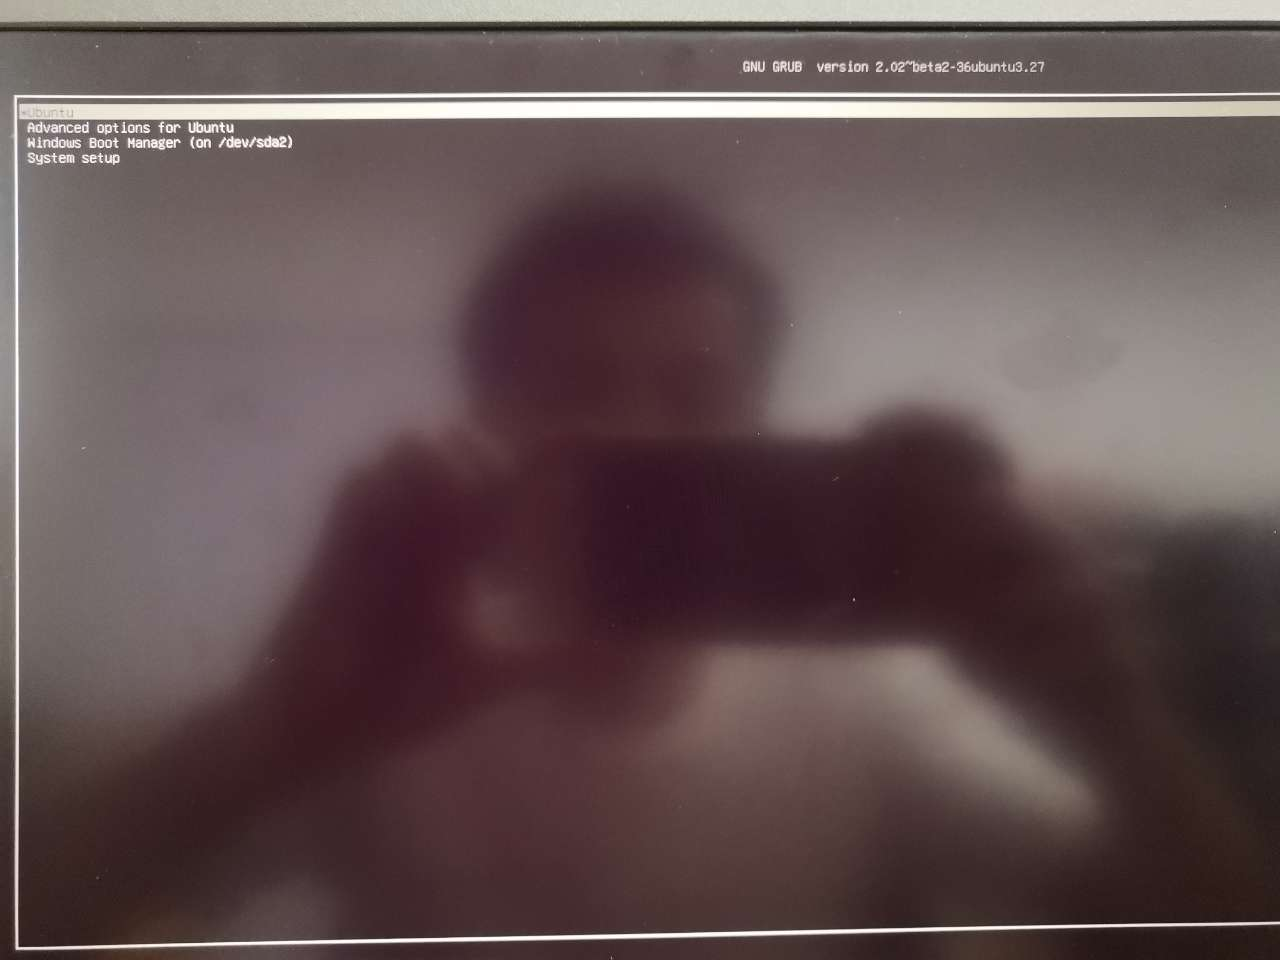
\includegraphics[width=5cm]{images/grub2_menu.jpg}
    \caption{GRUB2 启动菜单}
    \end{minipage}
    \end{figure}
\end{frame}

\begin{frame}[fragile]
    \frametitle{问题3:GRUB2 如何找到 Kernel?}
    /boot/grub/grub.cfg 记录各启动项的信息,根据该文件可找到 Kernel。以下为该文件的部分片段:

    \begin{lstlisting}[basicstyle=\tiny]
    menuentry 'Ubuntu' --class ubuntu --class gnu-linux --class gnu --class os
        $menuentry_id_option 'gnulinux-simple-fbd36807-5c5d-4a5e-b3cf-1ad135e9de5a' {
        set root='hd0,gpt6'
        if [ x$feature_platform_search_hint = xy ]; then
          search --no-floppy --fs-uuid --set=root --hint-bios=hd0,gpt6 --hint-efi=hd0,gpt6
              --hint-baremetal=ahci0,gpt6  e258e99d-ad24-4e57-8c8c-c549d455d717
        else
          search --no-floppy --fs-uuid --set=root e258e99d-ad24-4e57-8c8c-c549d455d717
        fi
        linux  /vmlinuz-4.15.0-122-generic root=UUID=fbd36807-5c5d-4a5e-b3cf-1ad135e9de5a ro  quiet splash $vt_handoff
        initrd  /initrd.img-4.15.0-122-generic
    \end{lstlisting}
\end{frame}

\begin{frame}
    \frametitle{问题4:initrd.img 是什么?有什么用?}

    \footnotesize
    \begin{itemize}
        \item initrd (initial ramdisk) is a scheme for loading a temporary root file system into memory, which may be used as part of the Linux startup process.
        \item This root file-system can contain user-space helpers which do the hardware detection, module loading and device discovery necessary to get the real root file-system mounted.
    \end{itemize}

    \begin{figure}[htbp]
    \centering
    \begin{minipage}[t]{0.48\textwidth}
    \centering
    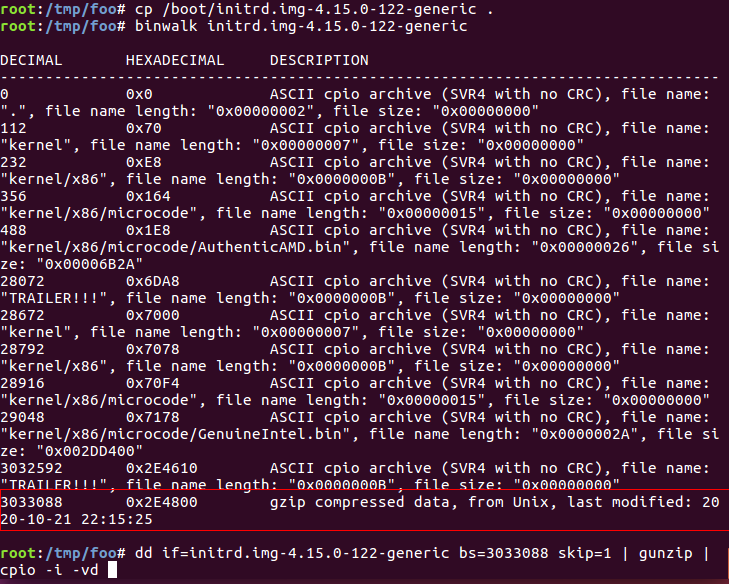
\includegraphics[width=3cm]{images/initrd_binwalk.png}
    \caption{initrd.img的内容}
    \end{minipage}
    \begin{minipage}[t]{0.48\textwidth}
    \centering
    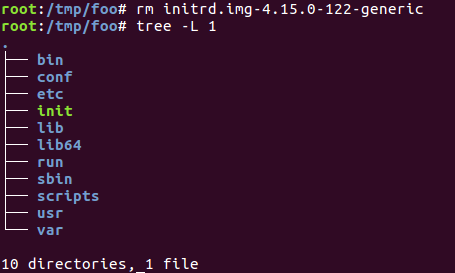
\includegraphics[width=3cm]{images/initrd_unpack.png}
    \caption{initrd.img解压后的内容}
    \end{minipage}
    \end{figure}
\end{frame}

\begin{frame}[fragile]
    \frametitle{Kernel 在内存中的布局}

    GRUB2 将 vmlinuz 分成2部分,实模式代码加载到内存中小于1M的位置,保护模式代码加载到不小于1M的位置。

    \begin{figure}[htbp]
    \centering
    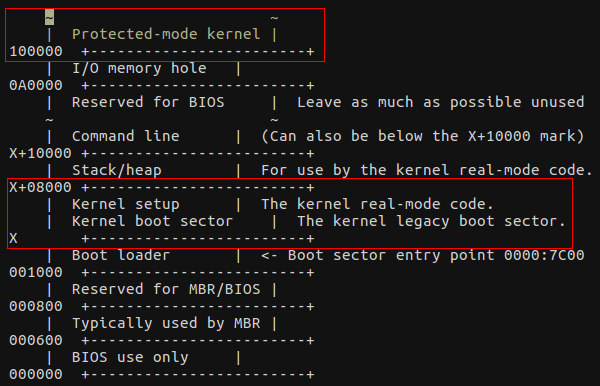
\includegraphics[width=6cm]{images/kernel_memory_layout.png}
    \caption{内核在内存中的布局}
    \end{figure}

\end{frame}

\begin{frame}
    \frametitle{x86 CPU 工作模式}

    \begin{itemize}
        \item 实模式
            \begin{itemize}
                \item 最大寻址空间为1MB
                \item 直接操作物理地址
                \item 只支持分段,不支持分页
                \item 不支持内存保护、多任务、特权级等
            \end{itemize}
        \item 保护模式
            \begin{itemize}
                \item 最大寻址空间为4GB
                \item 支持虚拟内存
                \item 支持分段和分页
                \item 支持内存保护、多任务、特权级等
            \end{itemize}
        \item 长模式
            \begin{itemize}
                \item 理论上最大寻址空间为$(2^{64})$,但目前一般在TB级别。
                \item 通用寄存器、指令指针、内存地址等都是64位。
            \end{itemize}
    \end{itemize}
\end{frame}

\section{Kernel}

\begin{frame}
    \frametitle{内核初始化流程}

    \begin{figure}
    \centering
    \begin{tikzpicture}[node distance=10pt]
        \node[startstop]                                       (start)   {GRUB2 将控制权交给 内核};
        \node[process, below=of start]                         (step 1)  {实模式 -> 保护模式 -> 长模式};
        \node[process, below=of step 1]                        (step 2)  {解压 vmlinuz};
        \node[process, below=of step 2]                        (step 3)  {体系结构初始化};
        \node[process, below=of step 3]                        (step 4)  {调度器初始化};
        \node[process, below=of step 4]                        (step 5)  {挂载 rootfs,并解压 initramfs 到 rootfs};
        \node[process, below=of step 5]                        (step 6)  {创建并运行第一个进程 /sbin/init(链接到systemd)};

        \draw[arrow] (start)  -- (step 1);
        \draw[arrow] (step 1) -- (step 2);
        \draw[arrow] (step 2) -- (step 3);
        \draw[arrow] (step 3) -- (step 4);
        \draw[arrow] (step 4) -- (step 5);
        \draw[arrow] (step 5) -- (step 6);
    \end{tikzpicture}
    \caption{内核初始化流程概览}
    \end{figure}
\end{frame}

\section{Init process}

\begin{frame}
    \frametitle{Systemd}

    \begin{itemize}
        \item 优点:功能强大,使用方便。
        \item 缺点:体系庞大,非常复杂。
    \end{itemize}

    \begin{figure}[htbp]
    \centering
    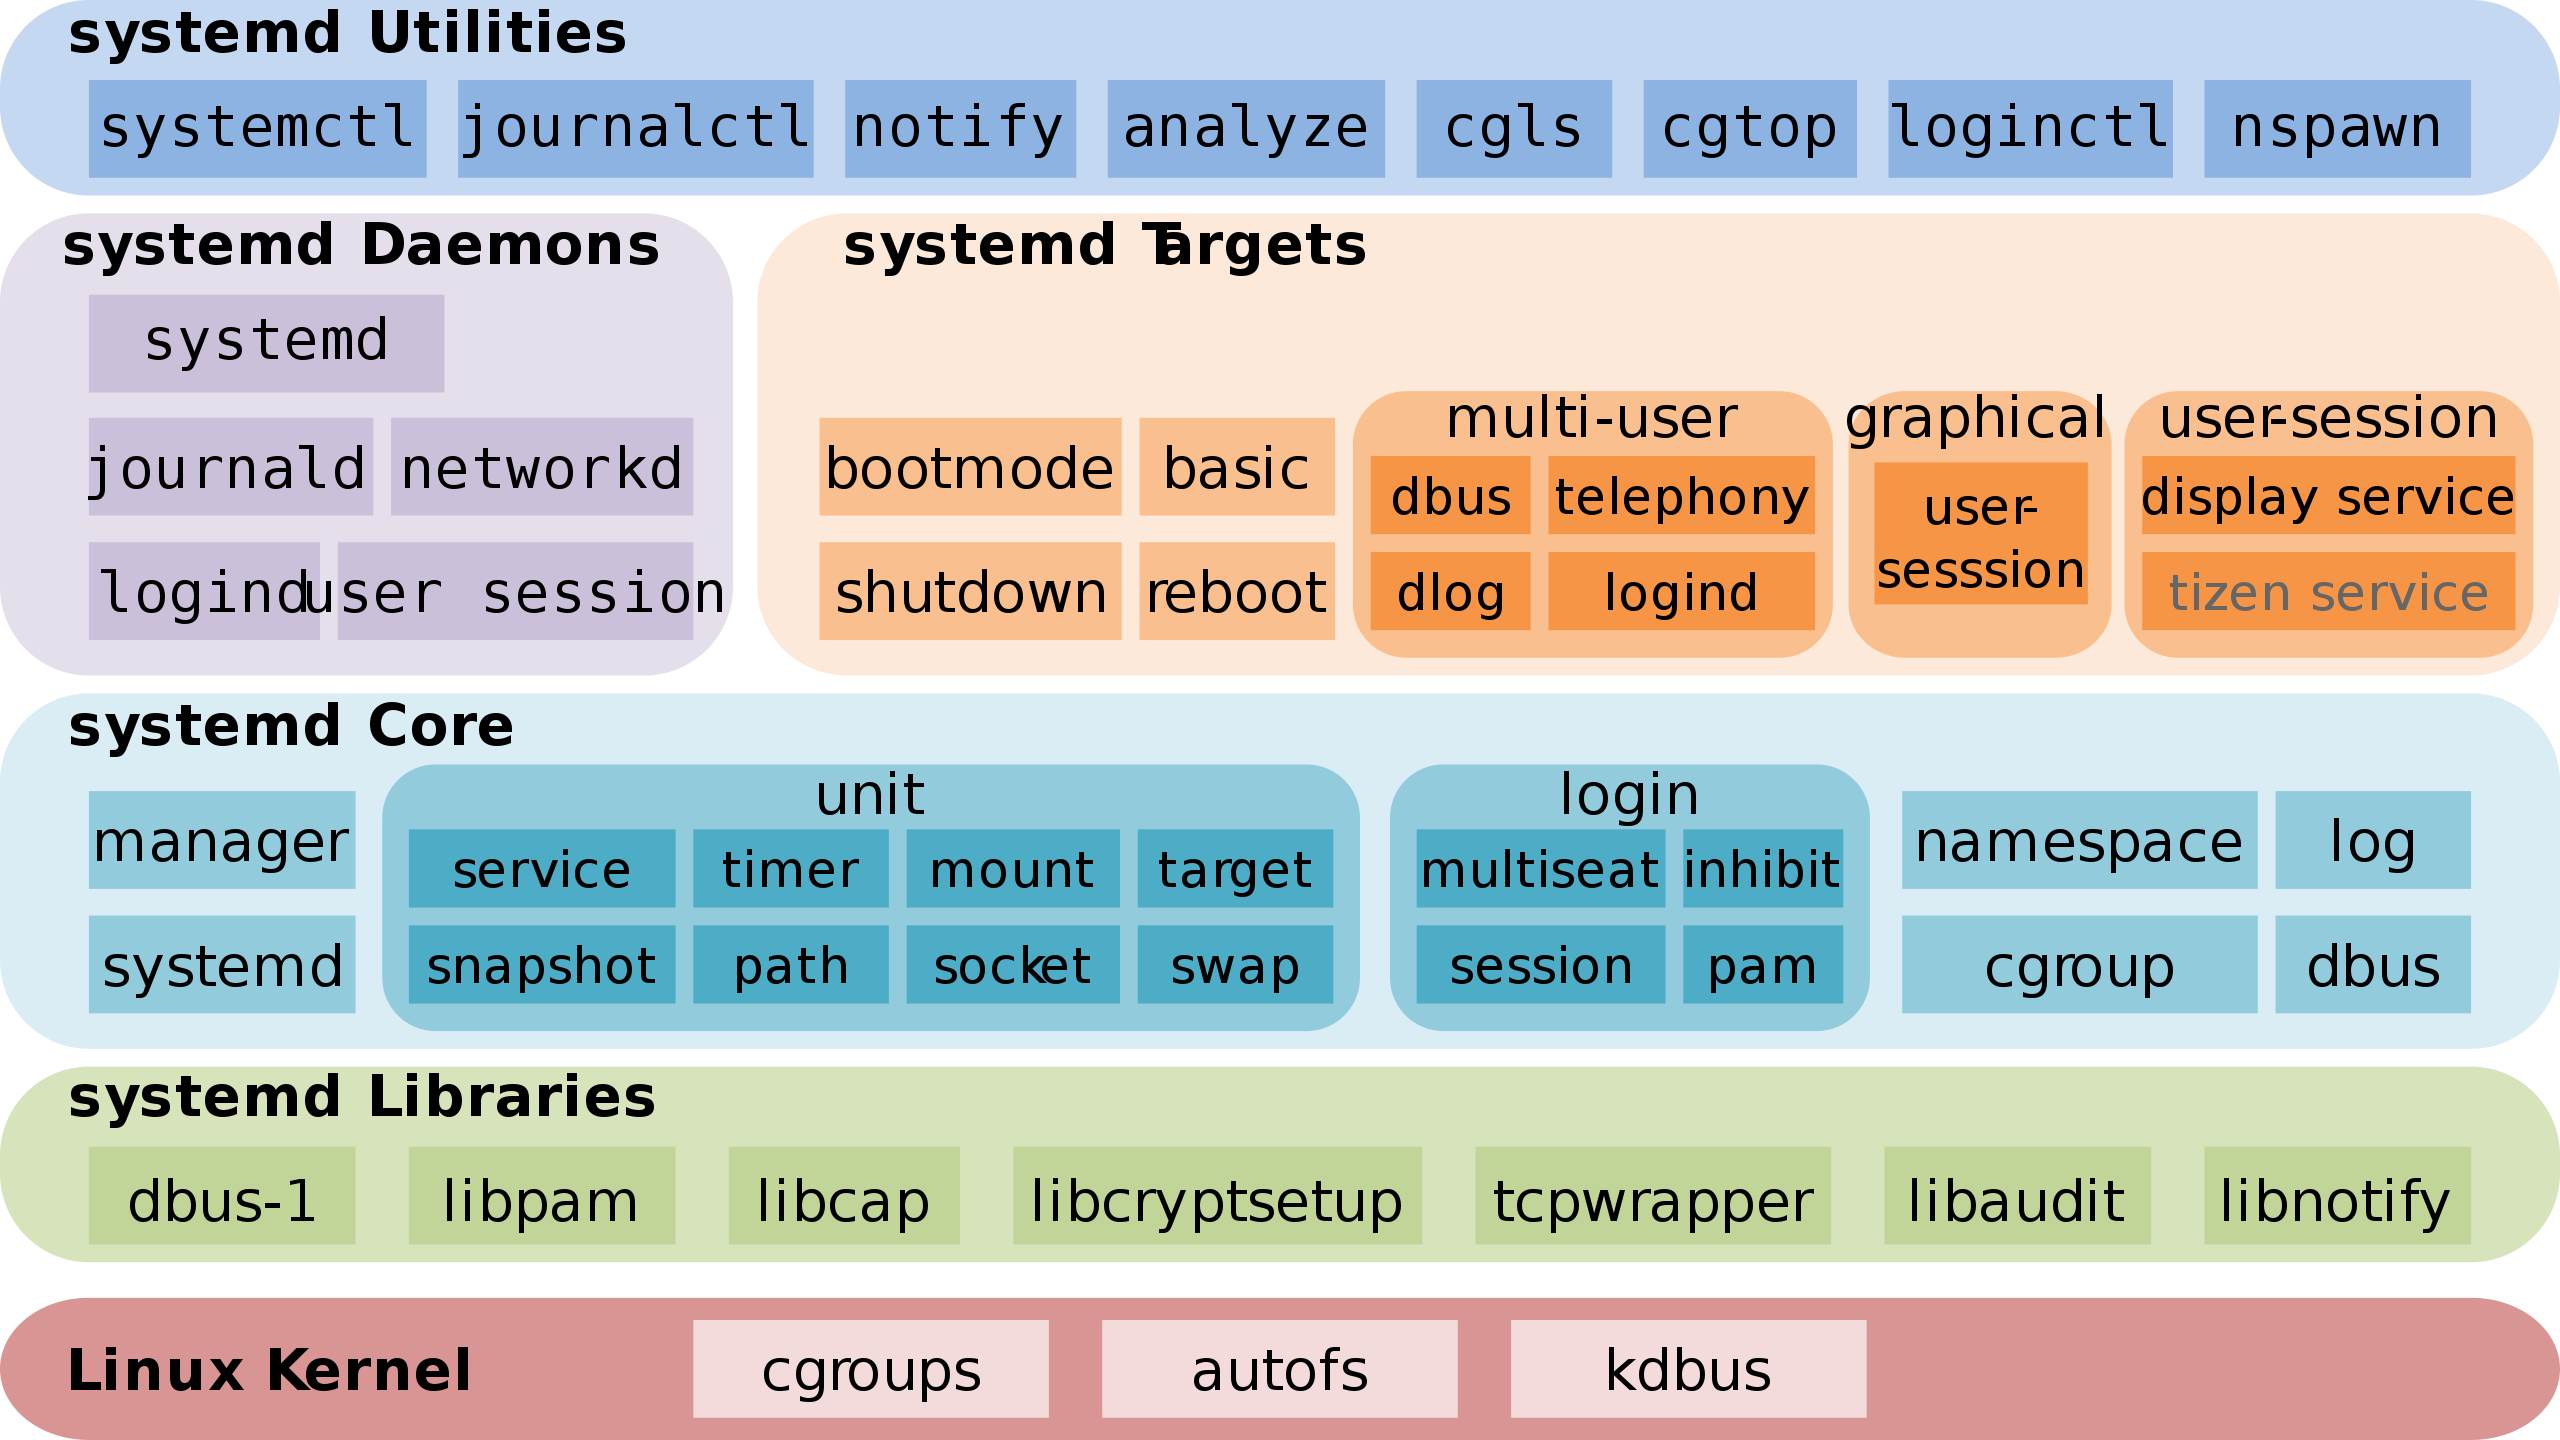
\includegraphics[width=6cm]{images/systemd_architecture.png}
    \caption{Systemd 架构}
    \end{figure}


\end{frame}

%------------------------------------------------

\begin{frame}
    \Huge{\centerline{\textcolor{blue}{Thank You}}}
\end{frame}

%----------------------------------------------------------------------------------------
\end{document}
